% draft 3rd-year diploma thesis, by Nick Manini, 2019/01/03
\documentclass[a4paper,12pt]{article}
\usepackage[english]{babel} % or other languages, e.g:
%\usepackage[italian]{babel} % needs debian package texlive-lang-italian
%\usepackage[latin1]{inputenc} % to use keyboard accented characters
\usepackage[a-1b]{pdfx} % to generate valid PDFA
                 % see https://www.mathstat.dal.ca/~selinger/pdfa/ for details
\usepackage{hyperref}
\usepackage{graphicx}
\usepackage{amsmath}
\usepackage{amssymb}
\usepackage{breakurl}
\usepackage{newtxtext}
\usepackage[varvw]{newtxmath}
\usepackage[width=0.8\textwidth]{caption}
\usepackage{booktabs}
\usepackage{geometry}
\usepackage{verbatim}
\usepackage{xmpincl}
\usepackage{appendix}
\usepackage{placeins}

% page size tuning:
\setlength{\oddsidemargin}{8mm}   % Distance from the left edge -1 inch
\setlength{\textwidth}{145mm}     % Horizontal width of the standard text
\setlength{\topmargin}{2mm}       % Distance from top to PAGE'S HEAD -1 inch
\setlength{\textheight}{225mm}    % Vertical length of the page body
\setlength{\headheight}{0mm}      % Height of a box containing the head
\setlength{\parskip}{0.5mm}       % Extra vertical space before a paragraph
\setlength{\parindent}{9mm}       % Indentation at paragraph beginning
\linespread{1.12}                 % Line-to-line spacing
\renewcommand{\floatpagefraction}{.95} % for text coexisting with figs and tabs
%\renewcommand{\textfraction}{0.02}% more or less equiv. to the above


%comandi veloci per le unità naturali
\newcommand{\f}[0]{\frac{V_0}{a}}
\newcommand{\g}[0]{\frac{1}{a}\sqrt{\frac{V_0}{m}}}
\newcommand{\p}[0]{\frac{V_0}{a^6}}
\newcommand{\tim}[0]{a\sqrt{\frac{m}{V_0}}}
\newcommand{\freq}[0]{\frac{1}{a}\sqrt{\frac{V_0}{m}}}
\newcommand{\vel}[0]{\sqrt{\frac{V_0}{m}}}



\begin{document}

\title{{\bf \huge
    Dynamical resonances in a bistable molecular model}}
\author{Alessandro Rizzi}
\date{October 6, 2021} % the exact date of graduation, when available

\makeatletter
\let\mytitle\@title
\let\myauthor\@author
\makeatother

\author{\myauthor \\
  Dipartimento di Fisica, Universit\`a degli Studi di Milano,\\
  Via Celoria 16, 20133 Milano, Italia
}

{ % heading page  -  frontespizio

  \thispagestyle{empty}

  \centerline{
    
\includegraphics[width=120mm,angle=0,clip=]{UniversitasMediolanensis.pdf}
  }

  \begin{center}
    {\Large Facolt\`a di Scienze e Tecnologie \\
      \vskip 2mm Laurea Triennale in Fisica }
  \end{center}


  \vskip 15mm
  \begin{center}
    \mytitle
%    \huge \textbf{Titolazzo della tesi, if seems long\\go to newline}
  \end{center}

  {\large
    \vskip20mm Relatore:  Prof. Nicola Manini
    \vskip 1mm Correlatore: Prof. Luciano Reatto\\
  }

  \vskip2cm
  \hskip9cm
  \parbox[t]{7cm}
         {\large 
           \myauthor\\
           Matricola n$^\circ$ $933340$\\
           A.A. $2020$/$2021$\\
           \vskip 0.5mm Codice PACS: 68.35.-p
         }

}


\clearpage
\thispagestyle{empty} \qquad

\maketitle \thispagestyle{empty}
\setcounter{page}{1}

%---------------------------------------------------------
\begin{abstract}
We study the one-dimensional dynamics of a bistable diatomic molecule driven across a sinusoidal periodic corrugation by a constant force. We investigate in detail the wide-amplitude motions of the internal molecular coordinate $r$, their relation with the effective driving force acting on $r$ and elucidate their mechanisms.
We also vary the driving force and other model parameters to address the resonances effects connected to the washboard frequency resulting from the sliding speed, both in the natural overdamped regime and in an hypothetical regime of weak damping. Finally, we evaluate the frictional contribution of the molecular dynamics.

\vskip0.75cm
\hskip5cm
\parbox[t]{7cm}
{
Advisor: {\it Prof. Nicola Manini}\\
Co-Advisor: {\it Prof. Luciano Reatto}
}
\end{abstract}
%--------------------------------------------------------

\clearpage
%\setlength{\oddsidemargin}{12mm}
\tableofcontents

\clearpage

%----------------------------------------------------------------------------
\section{Introduction}
%----------------------------------------------------------------------------

	%In this work we address the problem of the motion of a complex bistable diatomic biological molecule moving in an external corrugated potential, using the simplified model introduced in Ref.\cite{Cavallini}. The motion is studied in one dimension, leading to an especially simple, yet instructive, formulation of the problem, whose outcomes are expected to provide useful insights for the general three-dimensional motion.
This thesis can be considered as a prosecution of Ref.~\cite{Cavallini}. It focuses on the oscillations occurring in a regime of steady sliding of a diatomic molecule, pulled over a periodic corrugation by a constant force. The constituents of the molecule are bounded together by a bistable molecular potential. The motion is studied in one dimension, leading to an especially simple, yet instructive, formulation of the problem, whose outcomes are expected to provide useful insights for the general three-dimensional motion. In the present work we stick to zero temperature. Refs.~\cite{Fusco} and~\cite{Fasolino} deal with the effects of a finite temperature, but do not adopt a bistable internal potential. 

The model employed is described in Sec.~\ref{model:sec}. In Sec.~\ref{oscillations:sec} we provide an explication for the peculiar oscillations of the internal motion of the molecule, that spans from a local maximum to a local minimum of the molecular binding potential, already identified in Ref.~\cite{Cavallini}. In Sec.~\ref{resonances:sec} we discuss the applicability of a harmonic approximation for the oscillations in the molecular potential, and evaluate the extra friction that the molecule experiences when pulled over the periodic corrugation during steady advancement. While in Secs.~\ref{oscillations:sec} and~\ref{resonances:sec} we study the system in an overdamped regime, in Sec.~\ref{underdamped:sec} we give a brief overview of the oscillations occurring in the underdamped case. In Sec.~\ref{different:sec} we study the effects of a difference in the damping factor of the different constituents of the molecule on the internal oscillatory dynamics. In Sec.~\ref{conclusion:sec} we discuss the obtained results and some futures development of the problem. Finally, in Appendix~\ref{appendix:sec} is described the utilised numerical integration method.


\section{The model}\label{model:sec}

	\begin{figure}
\begin{center}
    \centering
    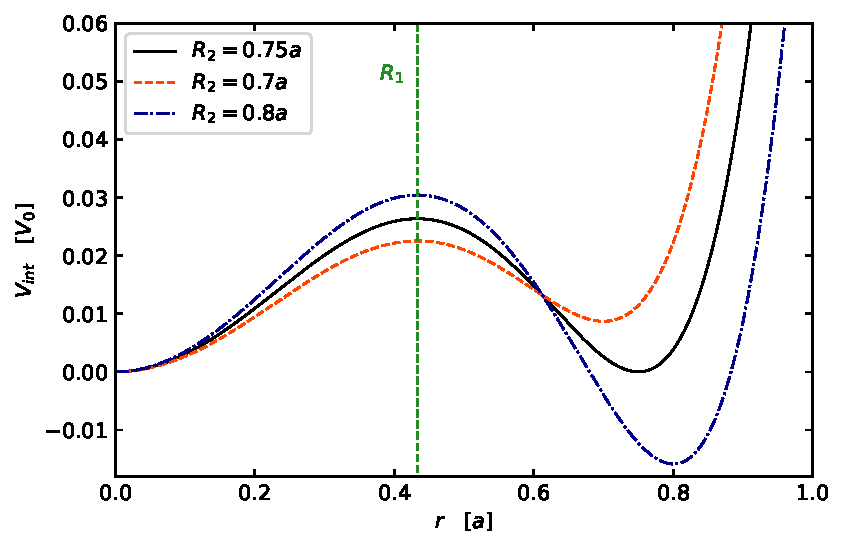
\includegraphics[width=1\linewidth]{Images/V_int.pdf}
    \caption{The molecular potential $V_\text{int}$ of Eq.~\eqref{eq:V_int} for fixed amplitude $U = 1 \p$ and location of the local maximum $R_1 = \frac{\sqrt{3}}{4} a$, and three different values of $R_2$. The first minimum is at the origin with null energy, the maximum is at $R_1$ and the second minimum at $R_2$.}
    \label{Fig:V_int}
\end{center}
\end{figure}

\begin{table}[]
    \centering
    \renewcommand\arraystretch{1.4}
    \begin{tabular}{c|c}
        \toprule
        Physical quantities &  Model units\\
        \midrule
        length             &   $a$   \\
        mass               &   $m$   \\
        energy             &   $V_0$  \\
        time               &   $\tim$   \\
        frequency and viscosity $\gamma$           &   $\freq$ \\
        force              &   $\f$    \\
        velocity           &   $\vel$  \\
        potential prefactor $U$        &   $\p$  \\
        \bottomrule
    \end{tabular}
    \renewcommand\arraystretch{1.2}
    \caption{All the relevant physical quantities for our work with their corresponding natural units}
    \label{tab:natural_units}
\end{table}


For the external corrugated potential $V_\text{ext}$ where the particles move we adopt the simplest periodic function:
\begin{equation}
    V_\text{ext}(x) = - \frac{V_0}{2}\cos\left(\frac{2\pi}{a}x \right), 
\end{equation}
where $V_0$ is the peak-to-peak energy amplitude, and $a$ is the period of the potential. We adopt the energy $V_0$, the length $a$ and the mass $m$ of each particle in the molecule as basic units, obtaining a system of natural units for the model, summarized in Table~\ref{tab:natural_units}. \\

The molecule is represented by two identical point-like particles of mass $m$ bounded together by a molecular bistable potential $V_\text{int}$ depending only on the distance between the particles. %The internal motion is so a one-dimensional problem, with only one degree of freedom.
The adopted analytical form of the potential has a first stable minimum at the origin at null energy, and a second minimum separated to the first by a barrier. The explicit expression is:
\begin{equation}
    V_\text{int}(r) = f( \zeta = r^2) = U\left[\zeta^3- \frac{3}{2}(R_1^2 + R_2^2)\zeta^2 + 3 R_1^2 R_2^2 \zeta \right],
    \label{eq:V_int}
\end{equation}
where $r = |x_2 - x_1|$ is the distance between the two particles, $U$ is a parameter that scales the strength of the potential, and $R_1$ and $R_2$ are the positions of the barrier and of the second stable minimum respectively, as sketched in Fig.~\ref{Fig:V_int}. Given that $R_1$ and $R_2$ have the dimension of a length, and so does $r$, $U$ must be an energy divided by a length to the sixth power. In general, the second minimum can be lower or higher in energy than the one at the origin, but if we select $R_2 = \sqrt{3}R_1$, it is at the same (zero) energy as the first minimum. Regardless of the fact that the minimum at $R_2$ can be either a local or an absolute minimum, in this work we will always refer to the potential barrier $\delta = V_\text{int}(R_1) - V_\text{int}(R_2)$. $\delta$ is the barrier that the molecule has to overcome to jump from the minimum at $R_2$ to the one at the origin. This definition is meaningful even when the origin is a local minimum and $R_2$ the absolute minimum because, practically, at null temperature and for equal drag coefficients on the two atoms, once the molecule is at zero, it has no chances of escaping to $R_2$. While the passage from zero to $R_2$ is not possible, the opposite usually is, and it may be fastened by the interaction of the molecule with $V_\text{ext}$. If $R_2 > \sqrt{3}R_1$, then $V_\text{int}(R_2) > 0$, and therefore the barrier $\delta$ is smaller than $V_\text{int}(R_1)$. On the contrary, if $R_2 < \sqrt{3}R_1$, then $V_\text{int}(R_2) < 0$ and $\delta > V_\text{int}(R_1)$. This can be easily verified by looking at the explicit expressions of $V_\text{int}(R_1)$, $V_\text{int}(R_2)$ and their difference:
\begin{align}
    \notag
    \delta = V_\text{int}(R_1) - V_\text{int}(R_2) = U\frac{R_2^6}{2}\left[ 3\left(\frac{R_1}{R_2}\right)^4 -  \left(\frac{R_1}{R_2}\right)^6 \right]
    -U\frac{R_2^6}{2}\left[ 3\left(\frac{R_1}{R_2}\right)^2 - 1\right] = \\
     = U\frac{R_2^6}{2}\left[ 1 -  \left(\frac{R_1}{R_2}\right)^6 + 3\left(\frac{R_1}{R_2}\right)^4  - 3\left(\frac{R_1}{R_2}\right)^2 \right].
    \label{eq:delta}
\end{align}
As can be seen, the magnitude of the potential barrier scales rapidly as $UR_2^6$\\


We shall now proceed to write the equations of motion. Starting from the full Hamiltonian of the system
\begin{equation}
    H = \sum_{i=1}^2 \left( \frac{p_{i}^2}{2m} + V_\text{ext}(x_i) - Fx_i \right) + V_\text{int}(|x_2 - x_1|),
\end{equation}
we obtain the classical Newton's law for the motion of the two particles:

\begin{align} 
    m \ddot{x}_{1}=F-\frac{V_{0} \pi}{a} \sin \left(\frac{2 \pi}{a} x_{1}\right)+ V'_\text{int}(r)-m \gamma \dot{x}_{1} \label{eq:x1},\\
    m \ddot{x}_{2}=F-\frac{V_{0} \pi}{a} \sin \left(\frac{2 \pi}{a} x_{2}\right)- V'_\text{int}(r)-m \gamma \dot{x}_{2}
    \label{eq:x2},
\end{align}
where 
\begin{equation}
    V'_\text{int}(r) = U\left[6\left(x_{2}-x_{1}\right)^{5}-6\left(x_{2}-x_{1}\right)^{3}\left(R_{1}^{2}+R_{2}^{2}\right)+6\left(x_{2}-x_{1}\right) R_{1}^{2} R_{2}^{2}\right],
\end{equation}
$F$ is the constant external force that we apply to the two particles. The dissipative term $m\gamma \dot{x}_{i}$ is non-Hamiltonian in nature, and must be adopted to dissipate the energy pumped in the system by the constant external force, and prevents states with constantly growing velocity. Thanks to this damping term we can obtain states with regular advancement, that are precisely what we plan to investigate. Physically, the $\gamma$ term accounts for the viscous friction that a real molecule is subject to when moving in a fluid.

The system is described by two coupled nonlinear ordinary differential equations (ODE), Eq.~\eqref{eq:x1} and~\eqref{eq:x2}. As we cannot see any exact analytical solution, we integrate these equations numerically by means of a Runge-Kutta-Fehlberg method, as descried in App.~\ref{appendix:sec}. The algorithm is capable of adjusting automatically the integration time step to maintain a prescribed accuracy~\cite{RKF45,RKF45_b}. Our code requires the specification of the following dynamical parameters of the model:
$R_1$, $R_2$, $U$, $F$, $\gamma$.
In addition, we need to set the initial conditions. We will call $R_0$ the initial value of $r =|x_2 - x_1|$. If not specified, the first particle is placed at the origin ($x_1=0, x_2 = R_0$), and both initial velocities are zero. 



\section{Oscillations covering the maximum at $R_1$ and the minimum at $R_2$}\label{oscillations:sec}

    \begin{figure}
\begin{center}
    \centering
    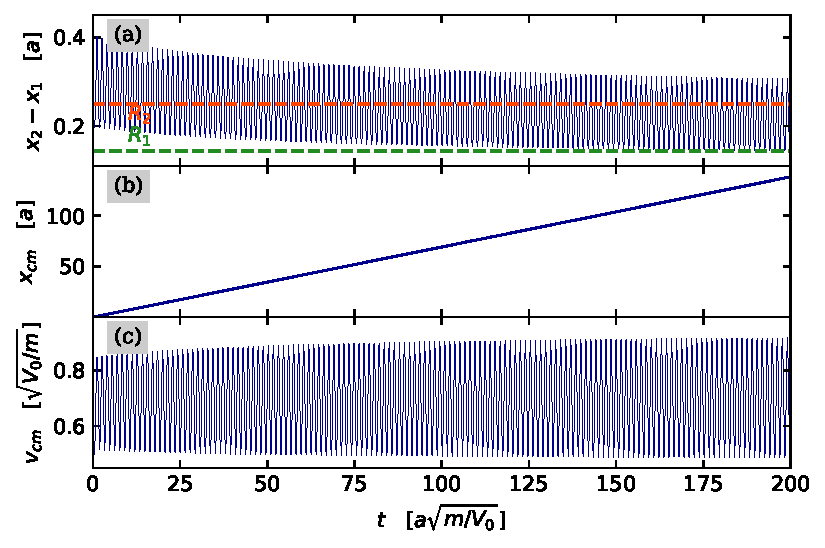
\includegraphics[width=1\linewidth]{Images/11_a_R_Xcm.pdf}
    \caption{Oscillations covering both the $R_1$ maximum and the $R_2$ minimum of the potential $V_\text{int}$, occurring with $R_1 = \frac{\sqrt{3}}{12} a$, $R_2 = 0.25 a$, $F = 7.5 \f$, $\gamma = 10 \g$, $ U = 1 \p$ and therefore $\delta = 3.6169 \times 10^{-5} V_0$ and initial condition $R_0=R_2$. \textbf{(a)} relative coordinate $r$; \textbf{(b)} center of mass $x_\text{cm}$; \textbf{(c)} velocity of the center of mass $v_\text{cm}$. }
    \label{Fig:11_a_R_Xcm}
\end{center}
\end{figure}

\begin{figure}
\begin{center}
    \centering
    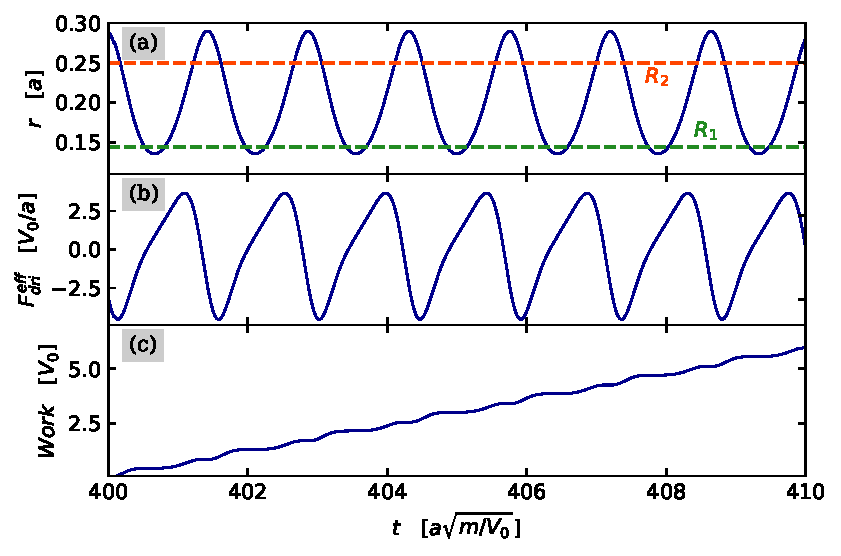
\includegraphics[width=1\linewidth]{Images/11_a_R_Forzante_2.pdf}
    \caption{\textbf{(a)} A blowup of a portion of the motion for the relative coordinate $r = |x_2 - x_1|$, as already reported in Fig.~\ref{Fig:11_a_R_Xcm}. \textbf{(b)} Effective driving force acting on this relative coordinate $F_{\text{dri}}^{\text{eff}}$, as given by Eq.~\eqref{eq:driving}. It can be seen that the force and the motion have the same frequency, and that the phase of the displacement is delayed by approximately 90° relative to the driving force. \textbf{(c)} Work of $F_{\text{dri}}^{\text{eff}}$. $W = \int_{t_0}^t F_{\text{dri}}^{\text{eff}}(t') \dot{r}(t') dt' $. We take $t_0 = 400 \tim$, safely after the initial non-periodic stage of the motion. }
    \label{Fig:11_a_R_Forzante}
\end{center}
\end{figure}


\begin{figure}
\begin{center}
    \centering
    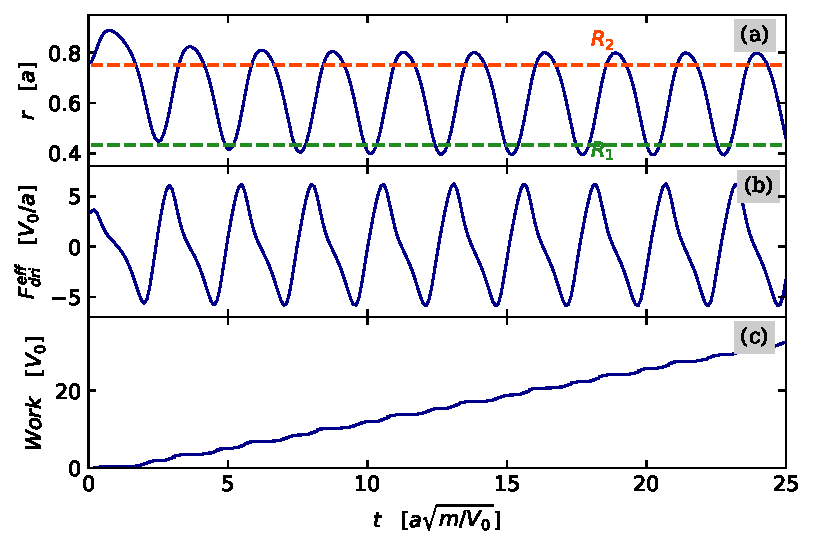
\includegraphics[width=1\linewidth]{Images/11_b_R_Forzante_2.pdf}
    \caption{Same as Fig.~\ref{Fig:11_a_R_Forzante} but with $R_1 = \frac{\sqrt{3}}{4} a$, $R_2 = \frac{3}{4} a$, $F = 5 \f$, $\delta = 2.6367 \times 10^{-2} V_0$, $R_0=R_2$. In panel \textbf{(c)} the work is integrated from $t_0 = 0 $.}
    \label{Fig:11_b_R_Forzante}
\end{center}
\end{figure}



Our first main objective is to identify an explanation for oscillations of the kind reported in Fig.~\ref{Fig:11_a_R_Xcm} and~\ref{Fig:11_b_R_Forzante} (a), also identified in Ref.~\cite{Cavallini}. These oscillations of the relative coordinate $r := |x_2 -x_1|$ are surprising because they seem not to be centered around a minimum of the molecular potential, but they span from a minimum to a local maximum, and even beyond it.

One can argue that the molecule has simply enough momentum to climb the potential barrier toward the maximum. However, this is not a valid argument for at least two reasons. The first one is that these oscillations are obtained in an overdamped regime, with $\gamma = 10 \g$.\footnote{A discussion about the values of $\gamma$ for which we can talk about an overdamped regime can be found in~\cite{Cavallini}, \S~4.1.} This large damping factor implies strong viscous friction, that makes all inertial movements rapidly disappear. This statement is confirmed by the second argument, i.e.\ that, as illustrated in Figs.~\ref{Fig:11_a_R_Forzante}a and~\ref{Fig:11_b_R_Forzante}a, the oscillation can extend even a little beyond the maximum at $R_1$. If inertia prevailed, then one would expect the molecule, once the barrier is climbed, to collapse to zero following the attractive force associated with $V_\text{int}$.

It must be now clear that a simple description based on a weakly driven oscillation around the minimum of $V_\text{int}$ is completely inadequate, and that is the motion along the periodic potential $V_\text{ext}$ that makes this peculiar behavior possible. A simple observation is that when $r$ has passed the maximum at $R_1$ and inverts his motion,
%mettere immagine chiara 
the two particles are found in different "valleys" of $V_\text{ext}$, i.e.\ the first is before one of the peaks, and the second is after. So the $x_1$ particle is pulled back to the left toward the previous minimum, and the $x_2$ particle is pushed forward. That favors an increase of their mutual distance $r$, that can effectively contrast the force generated by $V_\text{int}$. %magari formulare meglio: n esimo picco in na


But why do these oscillations occur only for some particular selections of the dynamical parameters? It is natural to require a reasonably small value of $\delta$ because if the forces generated by $V_\text{int}$ were too strong, it would be very difficult to climb the potential barrier and then not to collapse in the origin. Also, we already mentioned that a large damping factor helps quenching inertial effects. It is not trivial however to understand the role of $R_1$, $R_2$ and the external force $F$. We start by writing the Newton equation for the relative coordinate $r$:

%\begin{equation}
   % \mu\ddot{r} =  \overbrace{-\frac{V_0\pi}{a}\cos \left(\frac{2\pi x_\text{cm}}{a}\right)\sin\left(\frac{\pi r}{a}\right)}^{F_{\text{dri}}^{\text{eff}}} - V'_\text{int}(r) -2\gamma \mu \dot{r}
    %\label{eq:rdot}
%\end{equation}

\begin{equation}
    \mu\ddot{r} =  -\frac{V_0\pi}{a}\cos \left(\frac{2\pi x_\text{cm}}{a}\right)\sin\left(\frac{\pi r}{a}\right)- V'_\text{int}(r) -2\gamma \mu \dot{r},
    \label{eq:rdot}
\end{equation}
where $\mu = \frac{m_1m_2}{m_1+m_2}$ is the reduced mass of the molecule, that in our case of identical particles is equal to $m/2$. 
We can immediately make the following observations:
\begin{itemize}

    \item The motion of $r$ is coupled to that of the variable $x_\text{cm}$
    
    \item $F$ is not explicitly present in Eq.~\eqref{eq:rdot}, but it affects $r$ trough $x_\text{cm}$
    
    \item The $V'_\text{int}$ term is conservative, while the other force term
    \begin{equation}
         F_{\text{dri}}^{\text{eff}} :=-\frac{2V_0\pi}{a}\cos \left(\frac{2\pi x_\text{cm}}{a}\right)\sin\left(\frac{\pi r}{a}\right)
         \label{eq:driving}
    \end{equation}
    is responsible for pumping energy into the system. This energy is eventually dissipated by the final $\gamma$ term.
    
\end{itemize}


\begin{figure}
\begin{center}
    \centering
    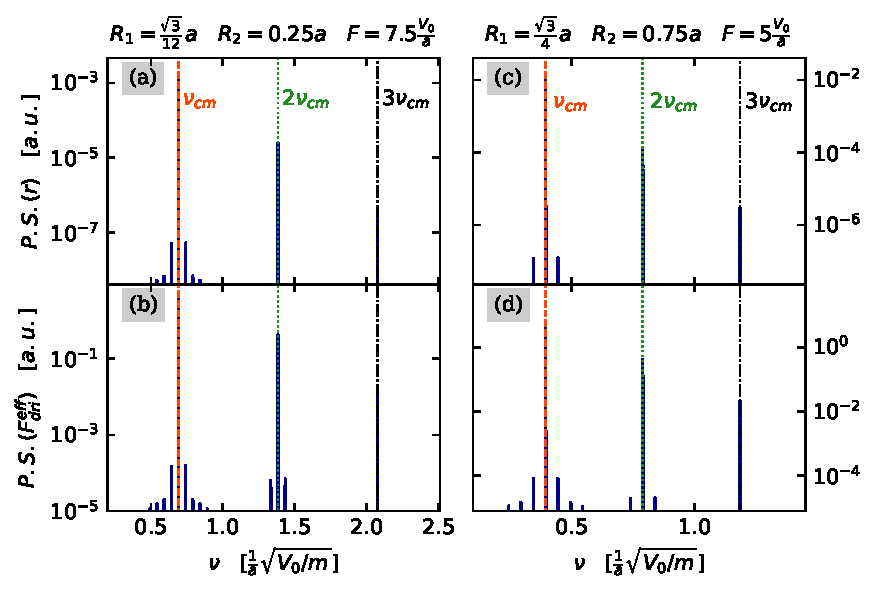
\includegraphics[width=1\linewidth]{Images/FFT.pdf}
    \caption{Power spectrum of the relative coordinate $r(t)$ and of the effective driving force $F_{\text{dri}}^{\text{eff}}(t)$ for the time sequences of: \textbf{(a)} Fig.~\ref{Fig:11_a_R_Forzante}a; \textbf{(b)} Fig.~\ref{Fig:11_a_R_Forzante}b; \textbf{(c)} Fig.~\ref{Fig:11_b_R_Forzante}a; \textbf{(d)} Fig.~\ref{Fig:11_b_R_Forzante}b. In all four spectra the peak corresponding to $\nu_\text{cm} = \Bar{v}_\text{cm}/a $ is dominant, followed by other weaker peaks at $2\nu_\text{cm}$ and $3\nu_\text{cm}$ representing the second and the third harmonic. Panels \textbf{(a,b)}:  $\nu_\text{cm} = 0.6927 \frac{1}{a}\sqrt{\frac{V_0}{m}}$; panels \textbf{(c,d)}:  $\nu_\text{cm} = 0.3950 \frac{1}{a}\sqrt{\frac{V_0}{m}}$.}
    \label{Fig:FFT}
\end{center}
\end{figure}

\begin{comment}
\begin{figure}
\begin{center}
    \centering
    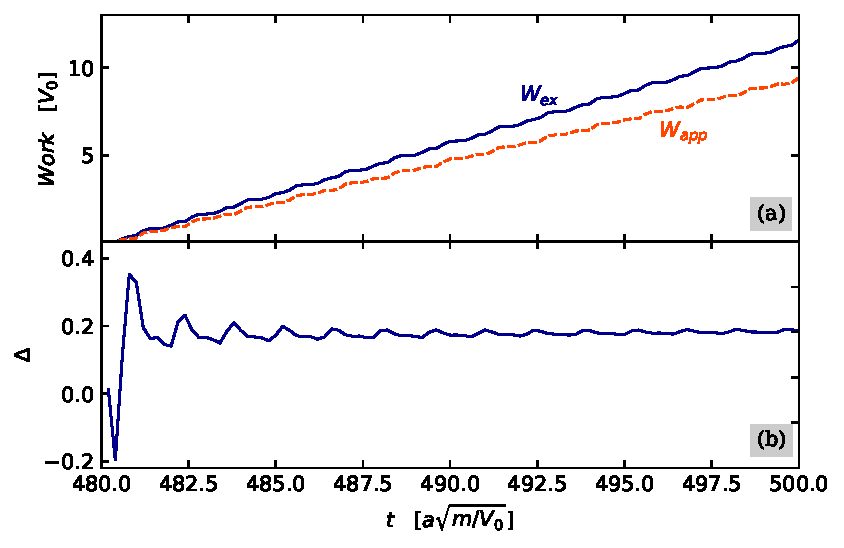
\includegraphics[width=1\linewidth]{Images/11_a_Work_b.pdf}
    \caption{Work of $F_{\text{dri}}^{\text{eff}}$ for the dynamics of Figs.~\ref{Fig:11_a_R_Xcm} and~\ref{Fig:11_a_R_Forzante}. $W = \int_{t_0}^t F_{\text{dri}}^{\text{eff}}(t') \dot{r}(t') dt' $. We take $t_0 = 480 \tim$, safely after the initial non periodic stage of the motion. \textbf{(a)} the solid line is the exact work $W_{ex}$, the dashed one is the approximate work $W_{app}$ obtained using the approximation of Eq.~\eqref{eq:coswt}; \textbf{(b)} relative error $\Delta = \frac{W_{ex}-W_{app}}{W_{ex}}$} 
    \label{Fig:11_a_Work}
\end{center}
\end{figure}

\begin{figure}
\begin{center}
    \centering
    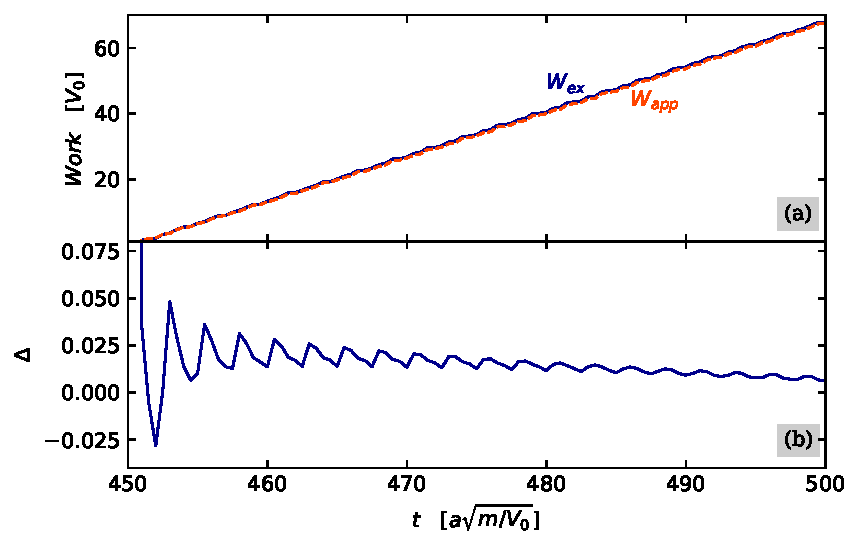
\includegraphics[width=1\linewidth]{Images/11_b_Work_b.pdf}
    \caption{Same as Fig.~\ref{Fig:11_a_Work} but for the oscillation of Fig.~\ref{Fig:11_b_R_Forzante} }
    \label{Fig:11_b_Work}
\end{center}
\end{figure}
\end{comment}

\subsection{The effective driving force}
We now focus on this effective driving force $F_{\text{dri}}^{\text{eff}}$, the force that drives these peculiar oscillations. Figures~\ref{Fig:11_a_R_Forzante} and~\ref{Fig:11_b_R_Forzante} show that, after the initial transient stage, the motion of $r$ oscillates at the same frequency of $F_{\text{dri}}^{\text{eff}}$, thus justifying the use of the term driving force. $F_{\text{dri}}^{\text{eff}}$ is the product of two oscillating terms, one dependent on $r$ itself and the other one on $x_\text{cm}$. Their combination can give rise to a complex time dependence of the effective force. Figures~\ref{Fig:11_a_R_Forzante}b and~\ref{Fig:11_b_R_Forzante}b show that $F_{\text{dri}}^{\text{eff}}$, after the initial transient stage, is a periodic function. 

We can first of all observe that (i) in a sliding (unpinned) state, $\cos \left(\frac{2\pi x_\text{cm}}{a}\right)$ spans all the values from -1 to +1; (ii) in the asymptotic oscillatory regime developed after the initial transient, if the oscillation is confined in a suitable limited region, $\sin\left(\frac{\pi r}{a}\right)$ ranges between $\sin\left(\pi\frac{ r_\text{min}}{a}\right)$ and $\sin\left(\pi\frac{ r_\text{max}}{a}\right)$, where $r_\text{min} \sim R_1$ and $r_\text{max} \sim R_2$ account for the oscillation range. For example, with the condition of Fig.~\ref{Fig:11_a_R_Forzante},
$ 0.39 < \sin\left(\frac{\pi r}{a}\right) < 0.81$; for the condition of Fig.~\ref{Fig:11_b_R_Forzante}, $ 0.59 < \sin\left(\frac{\pi r}{a}\right) < 0.95$. In these examples, this term never changes sign during the oscillation, and just modulates the main oscillatory term $\cos \left(\frac{2\pi x_\text{cm}}{a}\right)$. We can observe from Fig.~\ref{Fig:11_a_R_Xcm} (b,c) that the motion of $x_\text{cm}$ resembles a rectilinear uniform advancement, with small oscillations. Indeed $v_\text{cm}$ is not quite constant, but, after the initial transient, it oscillates around a mean constant value. If we neglect this small oscillation, we obtain the following approximation for this oscillatory term in $F_{\text{dri}}^{\text{eff}}$:
\begin{equation}
    \cos \left(\frac{2\pi x_\text{cm}}{a}\right) \approx \cos \left(\frac{2\pi \Bar{v}_\text{cm}}{a}t\right) = \cos\left(2\pi \nu_\text{cm}t\right) = \cos \left(\omega_\text{cm} t\right).
    \label{eq:coswt}
\end{equation}
In this equation, $\Bar{v}_\text{cm}$ is the mean velocity of the center of mass. Correspondingly, $\nu_\text{cm} = \Bar{v}_\text{cm}/a$ is the washboard frequency for the molecule advancing over the periodic corrugation. We then expect the frequency of $F_{\text{dri}}^{\text{eff}}$ and of the oscillation of $r$ to be exactly $\nu_\text{cm}$. This observation can be confirmed by a Fourier analysis. Figure~\ref{Fig:FFT} report the power spectrum, obtained as the squared modulus of its Fourier transform. The power spectrum of a quantity $y(t)$ is computed by
\begin{equation}
    P.S.(y)[\nu] = \left|\frac{1}{N}\sum_{n=1}^N e^{-2\pi i \frac{\nu n \Delta t}{N}}y[n \Delta t]\right|^2.
    \label{eq:ps}
\end{equation}
%This results in a peak in the origin for Fig.~\ref{Fig:FFT} (a) and (b), that is not reported.

%Another confirmation of the goodness of our approximation comes by looking at the energy pumped in the system by $F_{\text{dri}}^{\text{eff}}$, that we expect to be positive to balance the dissipation given by $\gamma \dot{r}$. In Figs.~\ref{Fig:11_a_Work} and~\ref{Fig:11_b_Work} are reported for both oscillations studied the work of the exact and approximate expression of $F_{\text{dri}}^{\text{eff}}$, and their normalized difference. The results are good in both cases, but especially for Fig.~\ref{Fig:11_b_Work}. For longer periods of integration the results can worsen significantly, because the approximate expression of $F_{\text{dri}}^{\text{eff}}$ can assume a different phase relative to $\dot{r}$, resulting even in an inversion of the trend of $W_{app}$, that starts decreasing.

\begin{figure}
\begin{center}
    \centering
    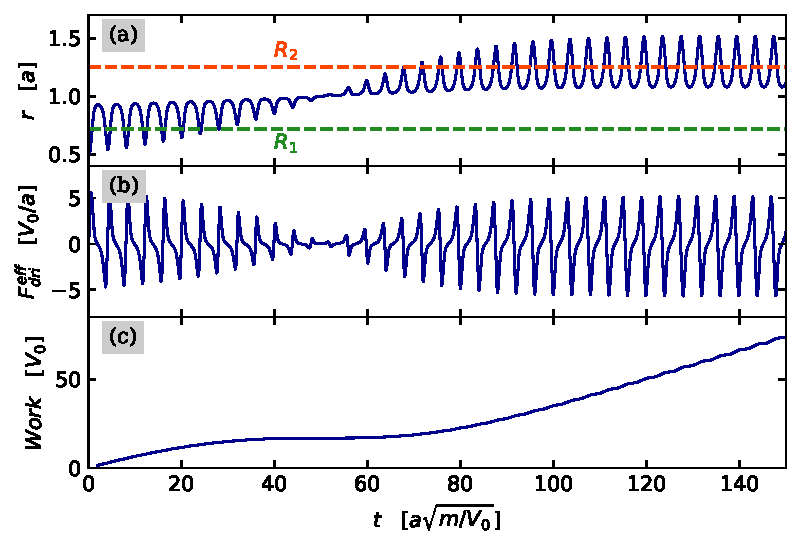
\includegraphics[width=1\linewidth]{Images/12_a.pdf}
    \caption{Example of dynamics in a condition where $R_1 < a < R_2$, implying a sign change of the $\sin \left(\frac{\pi r}{a}\right)$ term. $R_1 = 5\frac{\sqrt{3}}{12} a$, $R_2 = 1.25 a$,  $F = 4 \f$, $\gamma = 10 \g$, $ U = 0.01 \p$ (so that $\delta = 5.6514 \times 10^{-3} V_0$), initial condition $R_0= 0.5 a$. \textbf{(a)} relative coordinate $r$; \textbf{(b)} effective driving force $F_{\text{dri}}^{\text{eff}}$; \textbf{(c)} exact work done by $F_\text{dri}^{\text{eff}}$ on the internal degree of freedom. }
    \label{Fig:12_a}
\end{center}
\end{figure}

\begin{figure}
\begin{center}
    \centering
    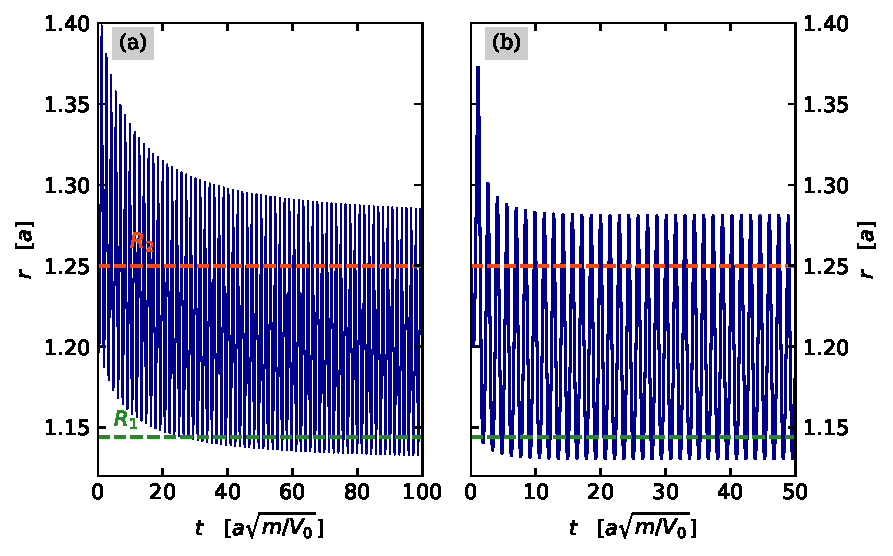
\includegraphics[width=1\linewidth]{Images/1.14434.pdf}
    \caption{Oscillations covering the maximum at $R_1 = 1.14434 a$ and the minimum at $R_2 = 1.25 a$. The simulation parameters are $\gamma = 10 \g$, $F = 7.5 \f$, and the initial condition is $R_0=R_2$. The other parameters are: \textbf{(a)} $U = 0.1 \p$ (so that $\delta = 8.0958 \times 10^{-4} V_0$); \textbf{(b)} $U = 1 \p$ ($\delta = 8.0958 \times 10^{-3} V_0$).}
    \label{Fig:1.14434}
\end{center}
\end{figure}

\begin{figure}
\begin{center}
    \centering
    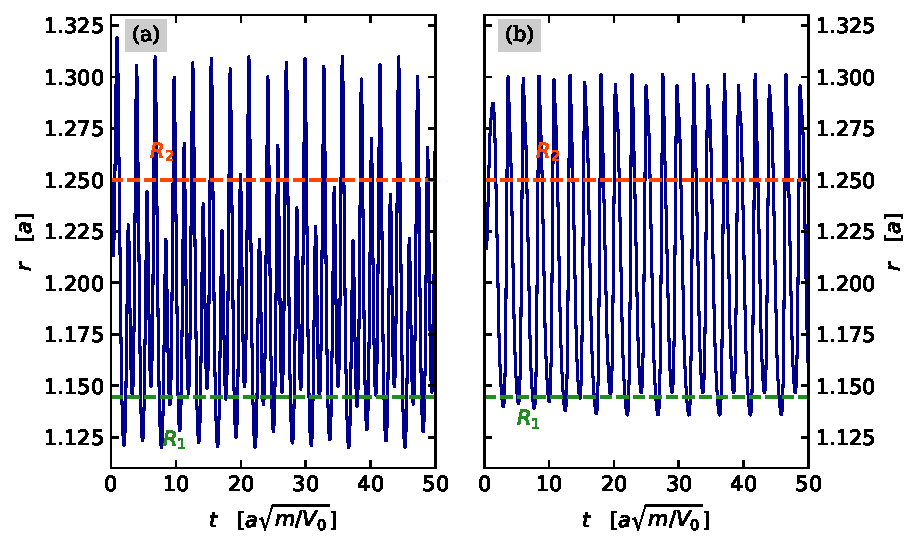
\includegraphics[width=1\linewidth]{Images/1.14434_b.pdf}
    \caption{Same as Fig.~\ref{Fig:1.14434}, but with \textbf{(a)} $F = 7.5 \f$, $U = 5 \p$ ($\delta =  4.0479\times 10^{-2} V_0$); \textbf{(b)} $F = 5.05 \f$, $U = 10 \p$ ($\delta =  8.0958\times 10^{-2} V_0$);}
    \label{Fig:1.14434_b}
\end{center}
\end{figure}

\subsection{Sign changes in $\sin(\pi r /a)$}
We are now convinced that $F_{\text{dri}}^{\text{eff}}$ plays a central role in driving the desired oscillations, and that the frequency of the latter is the same as the mean center of mass washboard frequency. From Figs.~\ref{Fig:11_a_R_Forzante}c and~\ref{Fig:11_b_R_Forzante}c, we can see that the work of $F_{\text{dri}}^{\text{eff}}$ is  monotonically increasing to sustain the oscillation. We then hypothesize that it helps that the term $\sin\left(\frac{\pi r}{a}\right)$ does not vanish nor change its sign during the oscillation. This is equivalent to ask that between $R_1$ and $R_2$ there are no points of the type $r = na$ with $n = 0, \pm1, \pm2 ...$

We investigate what happens when this condition is violated. Such a situation is reported in Fig.~\ref{Fig:12_a}. We see that when $r=a$, the effective driving force vanishes, and stops pumping energy into the molecule, leading to a small-amplitude oscillation in a neighborhood of $R_2$, where $F_{\text{dri}}^{\text{eff}}$ oscillates with sufficient amplitude. Thus a stable oscillation between $R_1$ and $R_2$ is not possible, and the oscillation around $R_2$ cannot extend beyond $r=a$, the point where $F_{\text{dri}}^{\text{eff}}$ vanishes.

As a limiting case, if we move this force-vanishing point to $R_2 = na$, no oscillations are sustained, and the molecule collapses to $R_2$, in a similar way as it collapses to the origin, giving a suitably small initial condition $R_0$. 

\subsection{Negative values of $\sin(\pi r /a)$}
We want to check what happens when the term $\sin\left(\frac{\pi r}{a}\right)$ assumes negative values. We then do a translation by $a$ of the spatial parameters $R_1$ and $R_2$ of the case of Figs.~\ref{Fig:11_a_R_Xcm} and~\ref{Fig:11_a_R_Forzante}. Doing so, the term $\sin\left(\frac{\pi r}{a}\right)$ is always negative between $R_1$ and $R_2$, with no vanishing points. For suitable values of $U$ and $F$, we observe the same kind of broad amplitude oscillation exceeding the maximum at $R_1$, as shown in Fig.~\ref{Fig:1.14434}. This proves that the sign of the term $\sin\left(\frac{\pi r}{a}\right)$ does not matter, as long as it remains the same during the entire oscillation. 

\subsection{Higher values of the potential barrier $\delta$}
We now want to check how the strength of $V_\text{int}$ affects the oscillations. We then proceed by increasing $U$, and therefore $\delta$, obtaining the desired oscillations until $U=10 \p$ and $\delta =  8.0958\times 10^{-2} V_0$. We can see however from Fig.~\ref{Fig:1.14434_b} that with this value of the barrier the oscillations follow more intricate patterns. Actually, after the initial transient, a Fourier analysis shows that their frequency is $\nu_\text{cm}/2$, corresponding to a period doubling, relative to the washboard period. These oscillations become more regular increasing the value of $F$, but their amplitude decreases with the driving force, so that eventually they cannot reach $R_1$. With a higher value of $U$ such as $15 \p$, corresponding to $\delta = 0.12144 V_0$ , $R_1$ is never reached. 
We noted that when $\delta$ increases, the minimum value of $F$ for which a stable oscillation can be established decreases. \\

Studying the oscillations covering both $R_1$ and $R_2$ presented in this section, we noted that after having reached a value of $F$ large enough to sustain these oscillations, if we further increase the external force, the amplitude of the oscillations decreases. Decreasing $F$, the oscillation switches with continuity from spanning over $R_1$ to remaining confined outside the barrier at $R_1$. We can therefore interpret these oscillations between the maximum and the minimum of $V_\text{int}$ as simple oscillations around the minimum at $R_2$, but with enough amplitude to climb the potential barrier at R1, as long as it is sufficiently weak.


%In general, for all the oscillations presented in this section, Here we have said that for increasing $F$, the amplitude of the oscillations becomes smaller and smaller. We will study in detail the dependence of the amplitude of an oscillation around $R_2$ on the external force in the next section. 
 
 %For the choice of dynamical parameters of Fig.~\ref{Fig:1.14434}, for forces smaller than $7.5 \f$, the system collapses in the origin after some oscillations, and for bigger forces, the oscillation around $R_2$ becomes smaller and smaller. The fact that   leads us to see these oscillations between the maximum and the minimum of $V_\text{int}$ as simple oscillations around the minimum at $R_2$, but with enough amplitude to climb the potential wall $\delta$ in case it is quite small.

\section{Near-$R_2$ oscillation resonances}\label{resonances:sec}

    %\captionsetup{width=0.9\textwidth,font=small}

As we now consider the oscillations between $R_1$ and $R_2$ as purely wide oscillations around the local minimum of $V_\text{int}$ at $R_2$, we are left with only two possible stable regimes in the overdamped case: either the molecule collapses to the origin, or a stable oscillation around $R_2$ is established. Focusing on the latter more interesting case, we recall the main result obtained in Section~\ref{oscillations:sec}, i.e.\\ that the driving frequency is the washboard frequency $\nu_\text{cm} = \frac{\Bar{v}_\text{cm}}{a}$. In addition, there is a relation between the external force $F$ and $\Bar{v}_\text{cm}$. In general, $\Bar{v}_\text{cm}$ grows when $F$ grows, but the exact dependence is non-trivial. In any case, we have an upper limit for the mean center-of-mass velocity, namely: $\Bar{v}_\text{cm} \leq F/m\gamma$. This means that the center of mass moves always more slowly than it would if it was not subject to any potential $V_\text{ext}$ or $V_\text{int}$. As we have previously mentioned, we observe that once the threshold value of $F$, for which a stable oscillation around $R_2$ is possible, is exceeded, the amplitude of such oscillation tends to decrease as $F$ and $\Bar{v}_\text{cm}$ increase. 

We now aim to study in a more rigorous way this trend, that might seem somewhat surprising. In fact, we expect to observe a peak in the amplitude of the oscillation when the washboard frequency approaches the natural oscillation frequency of the local minimum of $V_\text{int}$ at $R_2$. In the harmonic approximation this frequency is
\begin{equation}
   \nu_\text{harm} = \frac{\omega_\text{harm}}{2\pi} = \frac{1}{2\pi}\sqrt{\frac{V_\text{int}''(R_2)}{\mu}}.
   \label{eq:nu_harm}
\end{equation}

The evaluation of the second derivative of the internal potential at the minimum is straightforward and leads to

\begin{equation}
    V_\text{int}''(R_2) = 12U\left(R_2^4-R_1^2R_2^2 \right).
\end{equation}

To explore the possibility of resonances, we consider $R_1 = 1.5 a$ and $R_2 = 2.3 a$. We then change the external driving force $F$, and measure for each force the resulting peak-to-peak amplitude of the oscillations around $R_2$. We set $\gamma$ to $10 \g$, that is large enough to be in the overdamped case. The initial condition $R_0$ is set to $R_2$, in order to consistently trigger an oscillation around the minimum $R_2$, if possible. We then introduce the resonance velocity $v_\text{harm} = a\nu_\text{harm}$, for an easy comparison with $\Bar{v}_\text{cm}$. Figures~\ref{Fig:Resonance_a} and ~\ref{Fig:Resonance_b} report the oscillation amplitude obtained for a few values of $U$ (and therefore $\delta$ and $v_\text{harm}$). The black down-triangles in the plots represent the region before the depinning force, where the molecule does not move, and a blue circle marks an oscillation around $R_2$. In Fig.~\ref{Fig:Resonance_a}a, we see that for very small values of the potential barrier $\delta$, and thus of $v_\text{harm}$, once the oscillation is established, the amplitude decreases monotonically with $F$, in agreement with what was observed in Section~\ref{oscillations:sec}. In Fig.~\ref{Fig:Resonance_a} (c) and (d) we observe that when $\delta$ increases, a broad resonance peak appears. The peak becomes sharper and sharper as $U$ and thus $\delta$ increase, as reported in Fig.~\ref{Fig:Resonance_b}. Fig.~\ref{Fig:Resonance_5_b} is obtained with the same parameters as Fig.~\ref{Fig:Resonance_b}, but with a smaller damping factor $\gamma$. Here the resonance peaks are sharper, because the oscillator quality factor is larger~\cite{Mazzoldi}. %wikipedia https://en.wikipedia.org/wiki/Q_factor

\begin{figure}
\begin{center}
    \centering
    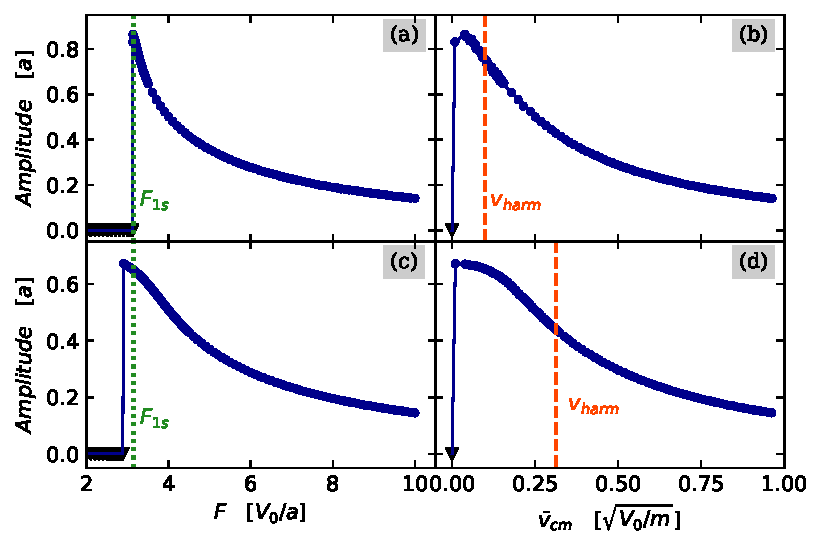
\includegraphics[width=1\linewidth]{Images/Resonance_2_a.pdf}
    \caption{The asymptotic oscillation amplitude $r_\text{max}-r_\text{min}$ as a function of \textbf{(a,c)} the applied force and \textbf{(b,d)} the resulting $\Bar{v}_\text{cm}$. The parameters are $R_1 = 1.5 a$, $R_2 = 2.3 a$, $\gamma = 10 \g$. The initial condition is $R_0=R_2$. The other parameters are: \textbf{(a,b)}: $U = 0.001 \p$ ($\delta = 1.4047 \times 10^{-2} V_0$); \textbf{(c,d)}: $U = 0.01 \p$ ($\delta = 0.14047 V_0$). The vertical dotted lines mark the static friction force $F_\text{1s}$ for one single free particle on $V_\text{ext}$. The vertical dashed lines mark the resonance velocities $v_\text{harm}$ corresponding to the harmonic frequencies for small amplitude oscillations near $R_2$. Panel \textbf{(b)}: $v_\text{harm} = 0.0989 \sqrt{V_0/m}$; panel \textbf{d}: $v_\text{harm} =  0.3127 \sqrt{V_0/m}$. The black triangles mark a value of $F$ below the depinning force, while the blue dots mark an oscillation around $R_2$. }
    \label{Fig:Resonance_a}
\end{center}
\end{figure}



\captionsetup{width=0.8\textwidth,font=normalsize}
\begin{figure}
\begin{center}
    \centering
    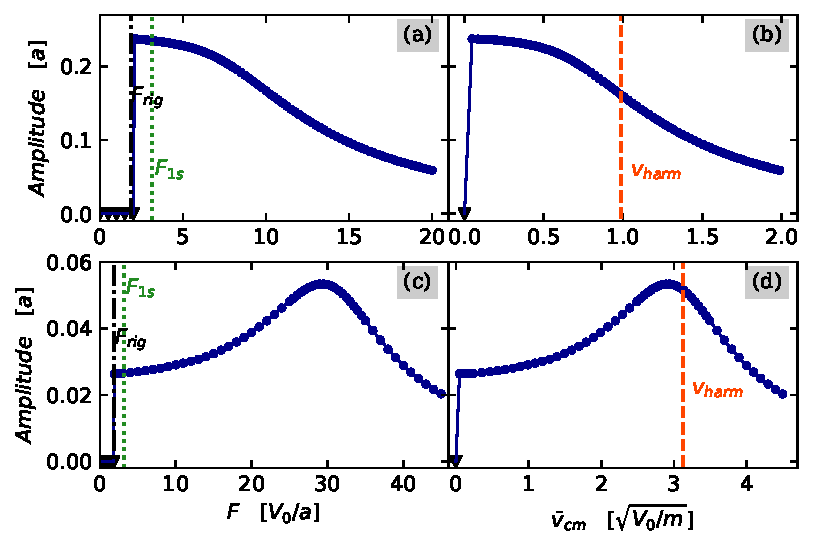
\includegraphics[width=0.85\linewidth]{Images/Resonance_2_b.pdf}
    \caption{Same as Fig.~\ref{Fig:Resonance_a}, but with stronger molecular potentials \textbf{(a,b)} $U = 0.1 \p$ ($\delta = 1.4047 \times 10^{-2} V_0$); \textbf{(c,d)} $U = 1 \p$ ($\delta = 14.047 V_0$). Panel \textbf{(b)}: $v_\text{harm} = 0.9888 \sqrt{V_0/m}$; panel \textbf{d}: $v_\text{harm} =  3.1267 \sqrt{V_0/m}$. The vertical dash-dotted lines mark the depinning force for a rigid molecule $F_\text{rig}$, where $r$ is fixed to $R_2$. }
    \label{Fig:Resonance_b}
\end{center}
\end{figure}


\begin{figure}
\begin{center}
    \centering
    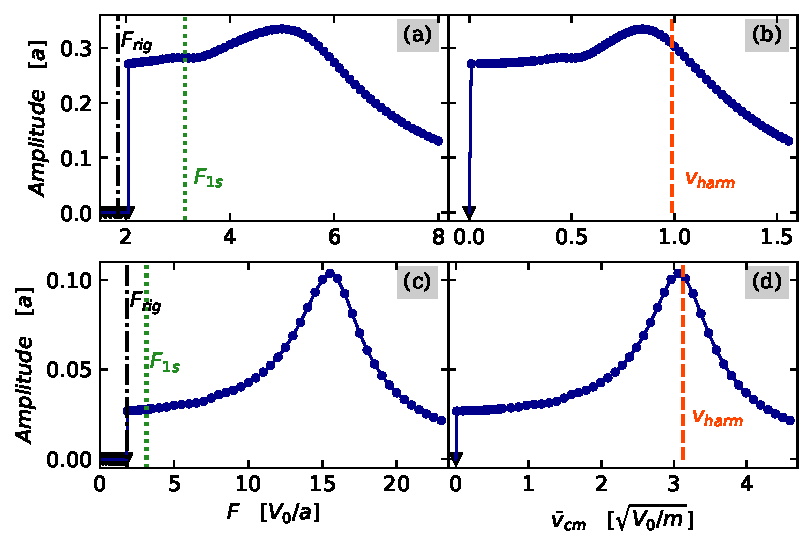
\includegraphics[width=0.85\linewidth]{Images/Resonance_b.pdf}
    \caption{Same as Fig.~\ref{Fig:Resonance_b}, but with $\gamma = 5 \g$}
    \label{Fig:Resonance_5_b}
\end{center}
\end{figure}


 

The picture is now clear: for small values of $\delta$, $V_\text{int}$ does not affect strongly the motion, the permitted oscillations around $R_2$ are wide, and a harmonic approximation of the phenomenon is meaningless. For increasing $\delta$, the forces generated by $V_\text{int}$ become stronger, the amplitude of the oscillations reduces and the harmonic approximation improves because the motion remains confined near the minimum.

For what concerns the value of the depinning force, we can see from Figs.~\ref{Fig:Resonance_a},~\ref{Fig:Resonance_b} and~\ref{Fig:Resonance_5_b}  (a,c) that it becomes smaller as $\delta$ increases. For very small $\delta$ the depinning force is almost the same as the static friction force for one free particle $F_\text{1s} = \pi \f$. When $\delta$ is larger, the depinning force decreases toward the depinning force for a rigid molecule where $r$ is fixed to $R_2$: $F_\text{rig} = \pi |\cos(\frac{\pi R_2}{a})| \f$. Clearly, $F_\text{rig} \leq F_\text{1s}$, so the bound exerted by $V_\text{int}$ helps the molecule to move on the external corrugated potential\footnote{A more exhaustive dissertation about the depinning force at various $U$ and $R_2$ can be found in Ref.~\cite{Cavallini}, \S~4.2.}.


\FloatBarrier
\subsection{Extra friction}

\begin{figure}
\begin{center}
    \centering
    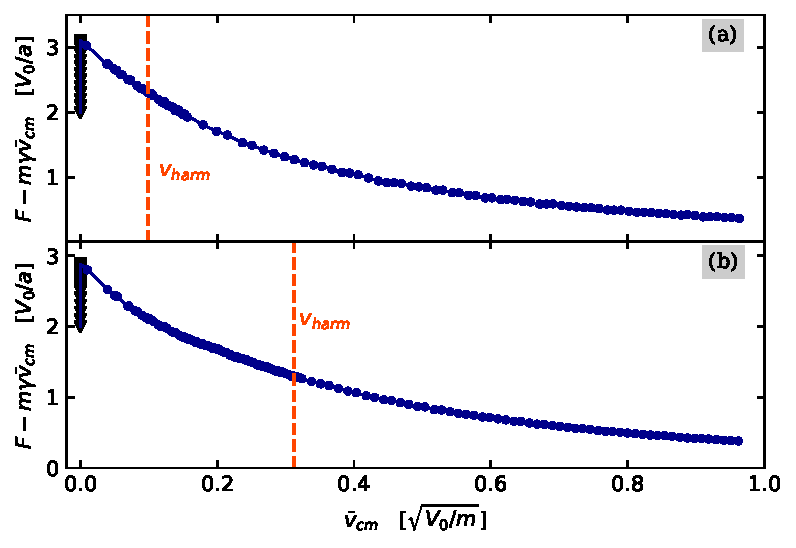
\includegraphics[width=1\linewidth]{Images/Attrito_2_a.pdf}
    \caption{Extra friction force for the molecule oscillating around $R_2$, as defined by Eq.~\eqref{eq:extra} as a function of the center-of-mass sliding velocity. \textbf{(a)} Same parameters as Fig.~\ref{Fig:Resonance_a} (a,b); \textbf{(b)} same parameters as Fig.~\ref{Fig:Resonance_a} (c,d).}
    \label{Fig:Attrito_a}
\end{center}
\end{figure}

\begin{figure}
\begin{center}
    \centering
    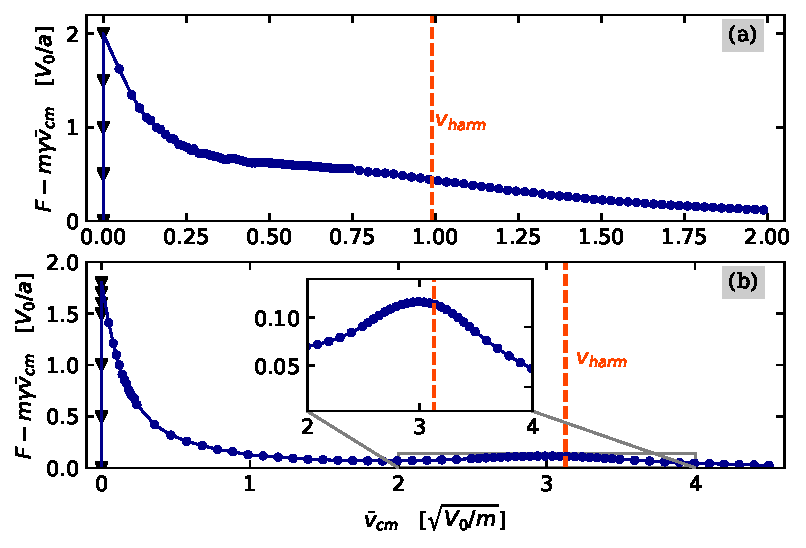
\includegraphics[width=1\linewidth]{Images/Attrito_2_b.pdf}
    \caption{Same as Fig.~\ref{Fig:Attrito_a} but: \textbf{(a)} same case as Fig.~\ref{Fig:Resonance_b} (a,b); \textbf{(b)} same case as Fig.~\ref{Fig:Resonance_b} (c,d).}
    \label{Fig:Attrito_b}
\end{center}
\end{figure}

\begin{figure}
\begin{center}
    \centering
    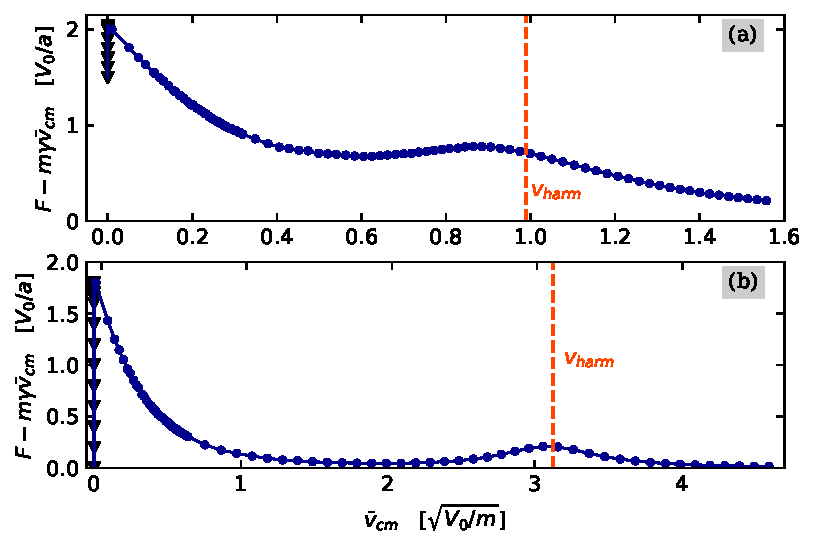
\includegraphics[width=1\linewidth]{Images/Attrito_b_2.pdf}
    \caption{Same as Fig.~\ref{Fig:Attrito_b} but wit $\gamma = 5 \g$.}
    \label{Fig:Attrito_5_b}
\end{center}
\end{figure}

We now aim to elucidate the extra friction, from now on abbreviated with e.f., originated from the molecule motions in a regime of steady advancement. We carry out a similar analysis as in Ref~\cite{Fusco} (where a pure harmonic molecular potential was adopted), adapting it to our model. We analyse the same oscillations studied in Figs.~\ref{Fig:Resonance_a} and~\ref{Fig:Resonance_b}, investigating how the e.f. varies with the strength of $V_\text{int}$. Figures~\ref{Fig:Attrito_a} and.~\ref{Fig:Attrito_b} report the e.f. force (per particle) that the molecule experience in addition to the trivial viscous friction force for a free particle in constant-velocity advancement at the same average velocity. The total average friction force exerted on the molecule (per particle) in a sliding scrolling regime, after the initial transient, is:

\begin{equation}
   \Bar{F}^{\text{tot}} = \frac{W^{\text{tot}}}{\Delta x} = \frac{1}{\Bar{v}_\text{cm}\tau} \int_{t_0}^{t_0+\tau}  F v_\text{cm}(t) dt =  \frac{F}{\Bar{v}_\text{cm}\tau} \int_{t_0}^{t_0+\tau}  v_\text{cm}(t) dt = F,
   \label{eq:tot}
\end{equation}
where $F$ is the force acting on one particle, $\Delta x = \Bar{v}_\text{cm}\tau$ is the total advancement path, $\int_{t_0}^{t_0+\tau}  v_\text{cm}(t) dt = \Bar{v}_\text{cm}\tau$ defines the average velocity, and $\tau$ is an integer number f periods of oscillation of the internal coordinate $r$. Recalling that a free particle pulled by a constant force $F$ moves with a terminal velocity $v_\text{cm}(t) = v_\text{free} = F/m\gamma $, the trivial friction force due to the free motion of the molecule (per particle) is:

\begin{equation}
   \Bar{F}^{\text{free}} = m \gamma \Bar{v}_\text{cm}.
   \label{eq:free}
\end{equation}

The extra friction force per particle is then
\begin{equation}
   \Bar{F}^{\text{extra}} = F - m\gamma \Bar{v}_\text{cm} = m\gamma (v_\text{free}-\Bar{v}_\text{cm}),
   \label{eq:extra}
\end{equation}
indicating that it measures the slowing down due to accelerations and decelerations of the center of mass and due to internal motions.

Figures.~\ref{Fig:Attrito_a} and~\ref{Fig:Attrito_b} report also the range where $F$ is insufficient to win the static friction, leading to $\Bar{v}_\text{cm} = 0$ (black down-triangles): here the molecule does not move, and Eqs.~\eqref{eq:tot} and~\eqref{eq:free} do not apply. After the depinning force, as long as the molecule starts to move, the e.f. is maximum, and then it decreases as the driving force force, and thus the sliding speed, increases. In the limit of large $F$, $\Bar{v}_\text{cm} \sim{\frac{F}{m\gamma}} $, i.e.\ for strong external force the perturbation induced by $V_\text{ext}$ and $V_\text{int}$ tends to become negligible, and the motion of the center of mass resembles that of a free particle.

In Fig.~\ref{Fig:Attrito_a}a, where $\delta = 1.4047 \times 10^{-2} V_0$, the e.f.\ decreases monotonically. Also in Fig.~\ref{Fig:Attrito_a}b, for a larger $\delta = 0.14047 V_0$, the e.f.\ decreases monotonically, but a very weak shoulder is observed for $\Bar{v}_\text{cm}$ near the harmonic velocity $v_\text{harm}$. This shoulder corresponds to the amplitude shoulder already reported in Fig.~\ref{Fig:Resonance_a}d. In Fig.~\ref{Fig:Attrito_b}b a proper peak in friction becomes visible as $\nu_\text{harm}$ increases. The friction peak is obviously related to the resonance peak in Fig.~\ref{Fig:Resonance_b}d. The peaks becomes again sharper when $\gamma$ is decreased, as reported in Fig.~\ref{Fig:Attrito_5_b}.

The physical explanation is simple: for increasing $\delta$ the amplitude of the oscillation reduces, the harmonic approximation becomes better and better and we observe an amplitude resonance peak when the frequency of the effective driving force approaches the natural oscillation frequency of $V_\text{int}$ around $R_2$. This peak in the amplitude of the oscillations induces a peak in the e.f. because part of the energy pumped into the molecule by $F$ is spent to sustain the motion of the relative coordinate $r$. We can also notice that $\Bar{F}^{\text{extra}}$ becomes generally smaller for larger $\delta$, again due to the amplitude of the $r$ oscillations decreasing with increasing rigidity of the molecule.

Eventually we recover the results obtained with a pure harmonic potential in Ref.~\cite{Fusco}, when we analyze oscillations around $R_2$ in the limit of small harmonic displacements. Our system is however more complex, because the harmonic approximation is valid only for quite large values of $V_\text{int}$, when the motion remains restricted to a small region around $R_2$. 
    
\section{The underdamped case}\label{underdamped:sec}

    \begin{figure}
\begin{center}
    \centering
    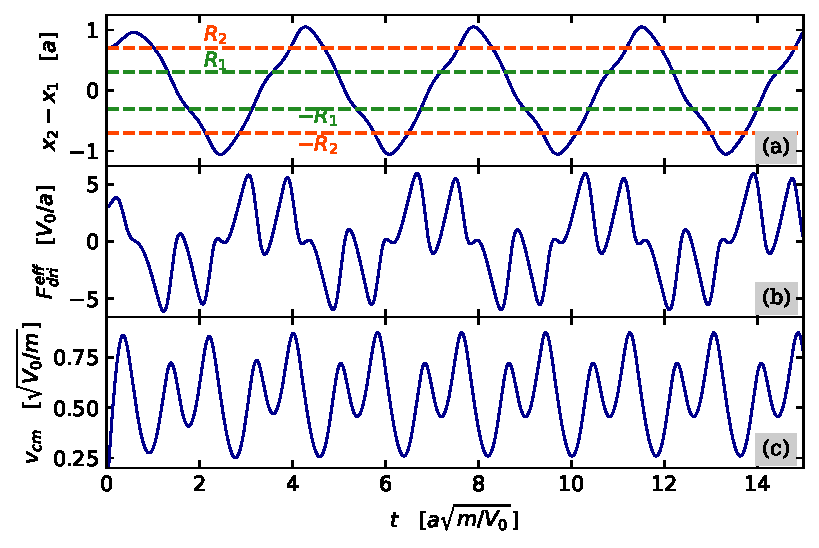
\includegraphics[width=1\linewidth]{Images/Underdamped.pdf}
    \caption{Oscillations in the underdamped case with $R_1 = 0.3 a$, $R_2 = 0.7 a$, $F = 2.6 \f$, $\gamma = 2 \g$, $ U = 1 \p$ ($\delta = 3.1999 \times 10^{-2} V_0$) and initial condition $R_0=R_2$. \textbf{(a)} relative coordinate $r$; \textbf{(b)} effective driving force $F_\text{dri}^\text{eff}$; \textbf{(c)} velocity of the center of mass $v_\text{cm}$. }
    \label{Fig:Underdamped}
\end{center}
\end{figure}

\begin{figure}
\begin{center}
    \centering
    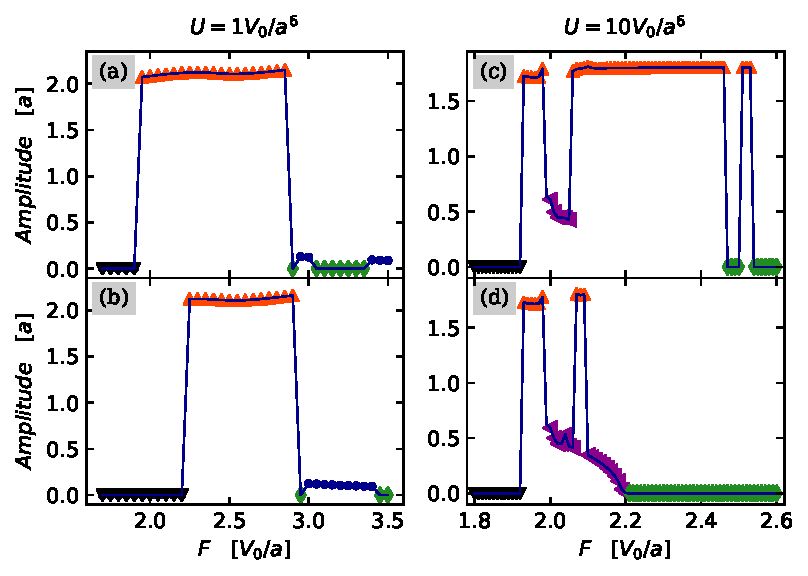
\includegraphics[width=1\linewidth]{Images/Underdamped_res_col.pdf}
    \caption{Oscillation amplitude $r_{max}-r_{min}$  as a function of $F$ for $R_1 = 0.3 a$, $R_2 = 0.7 a$, $\gamma = 2 \g$. \textbf{(a,b)}:  $ U = 1 \p$ ($\delta = 3.1999 \times 10^{-2} V_0$); \textbf{(c,d)}:  $ U = 10 \p$ ($\delta = 0.31999  V_0$). In panels \textbf{(a,c)} the initial condition is $R_0=R_2$; in panels \textbf{(b,d)} $R_0=a$. The red up-triangles mark oscillations with amplitude $A > 2R_2$, the green diamonds mark a collapse to the origin, and the purple left-triangles indicate an oscillation around the origin.}
    \label{Fig:Underdamped_res}
\end{center}
\end{figure}

\begin{figure}
\begin{center}
    \centering
    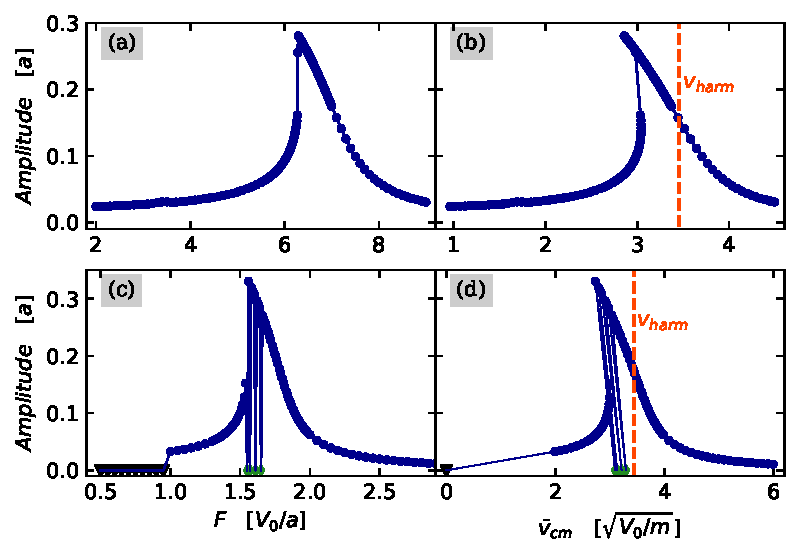
\includegraphics[width=1\linewidth]{Images/Underdamped_res_2_col.pdf}
    \caption{Effects of changing $U$ and $\gamma$. Amplitude of the oscillations for $R_1 = 0.3 a$, $R_2 = 0.7 a$, $ U = 100 \p$ ($\delta = 3.1999  V_0$) and initial condition $R_0=R_2$ and \textbf{(a,b)}: $\gamma = 2 \g$; \textbf{(c,d)}: $\gamma=0.5 \g$.}
    \label{Fig:Underdamped_res_2}
\end{center}
\end{figure}

\begin{figure}
\begin{center}
    \centering
    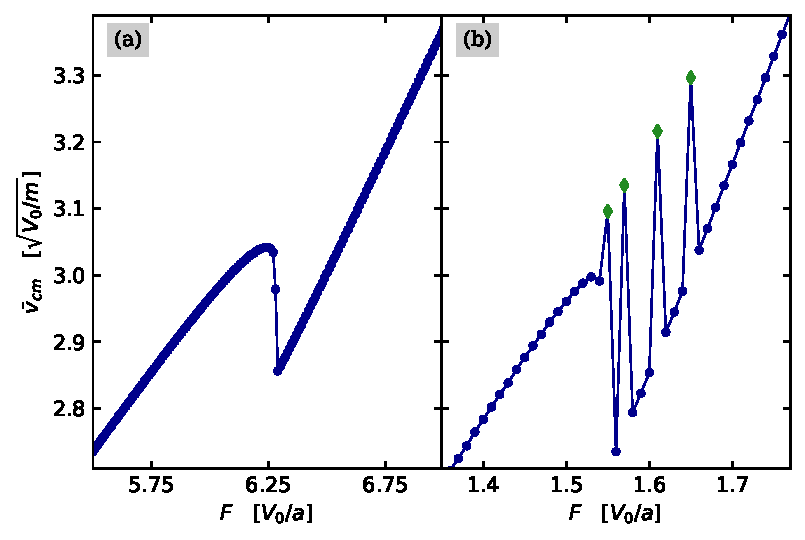
\includegraphics[width=1\linewidth]{Images/Bistability_2.pdf}
    \caption{Bistabilities of the underdamped dynamics. \textbf{(a)} Same parameters as Fig.~\ref{Fig:Underdamped_res_2} (a,b); \textbf{(b)} same parameters as Fig.~\ref{Fig:Underdamped_res_2} (c,d). The green diamonds mark a collapse at the origin.  }
    \label{Fig:Bistability}
\end{center}
\end{figure}


So far we focused on overdamped dynamics. In this section, we provide a brief overlook of the behavior of the underdamped molecule, keeping in mind that this regime is less likely to be relevant in practice. 

As shown in Fig.~\ref{Fig:Underdamped}, if $\delta$ is moderate and for small external forces $F$, a small damping produces very wide oscillations and an extremely short initial transient. The main novelty of the underdamped case is that $r$ can pass through zero without collapsing permanently there. This is possible because when $r$ passes trough the origin it carries enough momentum to escape the $r=0$ basin even if $F_\text{dri}^\text{eff}$ vanishes. Figure~\ref{Fig:Underdamped}b shows that $F_\text{dri}^\text{eff}$ vanishes every time that $r$ passes trough $0$ or $\pm a$ due to the term $\sin\left(\frac{\pi r}{a}\right)$, plus other two times due to the normal oscillation of the $\cos\left(\frac{2\pi x_\text{cm}}{a}\right)$ term. This results in a fairly intricate time dependence of $F_\text{dri}^\text{eff}$, and as a consequence the oscillation of $r$ involves a complicated pattern with several Fourier components. Figure~\ref{Fig:Underdamped}c shows that $v_\text{cm}$ too is far more complicated than a simple sinusoid. Anyway the fundamental frequency of the oscillation of $r$ and of $F_\text{dri}^\text{eff}$ is still the washboard frequency $\nu_\text{cm}$. For high values of $F$ the two well-known features of steady sliding are retrieved: the collapse to the origin and the ordinary oscillations around $R_2$, or around $-R_2$, because the particles can occasionally swap during the initial transient.

\subsection{Resonances}
To  better understand the dependence of these wide oscillations on the external force, we carry out for the underdamped system the same analysis as we did in Sec.~\ref{resonances:sec} for the overdamped molecule. Here we obtain quite different results. Figure~\ref{Fig:Underdamped_res} shows that the $F$-dependence of the oscillation amplitude is more complex and discontinuous than in the overdamped case. That is because in the latter, after the depinning force, we only had regular oscillations around $R_2$, which provide a smooth resonant behaviour. Here, on the contrary, we observe the alternation of several kinds of oscillations, one of which being exemplified Fig.~\ref{Fig:Underdamped}, and that can depend crucially on the initial condition.

We can divide Figs.~\ref{Fig:Underdamped_res} (a,b) in three ranges of applied force $F$, where different kinds of oscillation occur. Starting from small $F$, in the first range the molecule does not move, i.e.\ $F$ is below the depinning force (black down-triangles). Increasing $F$, we observe a plateau of very wide oscillations with amplitude $A > 2 R_{2}$ of the kind reported in Fig.~\ref{Fig:Underdamped} (red up-triangles). For even larger forces, we retrieve either small-amplitude oscillations around $R_2$ (blue circles) or a collapse to the origin (green diamonds), resulting in a null value of the amplitude. The comparison of panel (a) with panel (b) shows that where these regions begin and end depends on the starting condition $R_0$. Figure~\ref{Fig:Underdamped_res} (c,d), where $\delta$ is larger, reports even more complicated patterns. The oscillations with a smaller amplitude that interrupt the plateau are oscillations around the origin (purple left-triangles). This is a completely new kind of oscillation, that cannot occur in the overdamped system. In some cases, these oscillations are clean periodic oscillations around a minimum, but for some values of $F$, we even observe intricate quasi-periodic patterns.

In Fig.~\ref{Fig:Underdamped_res_2} (a,b), where we increase $U$ to  $100\p$ (so that $\delta=3.1999  V_0$), we see that a resonance peak near the harmonic frequency arises.  In Fig.~\ref{Fig:Underdamped_res_2} (c,d) we decrease $\gamma$ to $0.5\g$, and we observe that the resonance peak is interrupted by a few collapses to the origin (green diamonds). That is because with such a small damping factor, near the resonance, the oscillation extends beyond $R_1$, but then the $r=0$ minimum can sometimes capture the motion, because wide oscillations across the origin are disfavoured by the high barrier $\delta$. Panels (b,d) show a dynamical bistability near the resonance, i.e.\ the same center-of-mass velocity is obtained for different values of $F$. These instabilities are shown in more detail in Fig.~\ref{Fig:Bistability}. The same result for an underdamped dimer was observed in Ref.~\cite{Fusco}. 

In general, the underdamped dynamics exhibits a larger variety of oscillations, and is far more sensitive to the initial condition than the overdamped case.    
    
\section{Different damping of the two atoms}\label{different:sec}

    \begin{figure}
\begin{center}
    \centering
    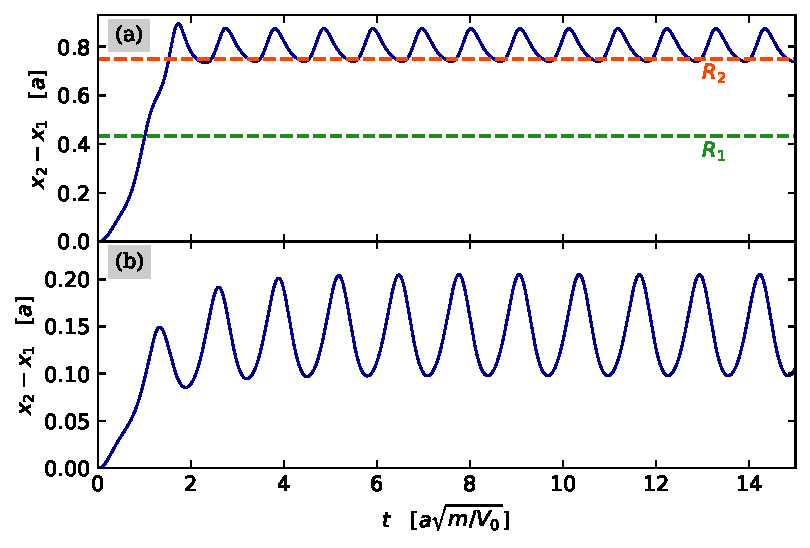
\includegraphics[width=1\linewidth]{Images/different.pdf}
    \caption{Oscillations with different damping factors for the two particles. $R_1 = \frac{\sqrt{3}}{4} a$, $R_2 = 0.75 a$, $ U = 10 \p$ (and therefore $\delta = 0.2637 V_0$), $F = 7.5 \f$, $\gamma_1 = 10 \g$ and initial condition $R_0=0$. \textbf{(a)} $\gamma_2 = 0.5 \gamma_1$; \textbf{(b)} $\gamma_2 = 0.8 \gamma_1$.  }
    \label{Fig:different}
\end{center}
\end{figure}

In this section we study how the system changes when the symmetry between the two particles $x_1$ and $x_2$ is broken, by taking two different damping factors that we call $\gamma_1$ and $\gamma_2$, respectively. This means that now the units forming the molecule are different, as could occur in a real physical system. 

For simplicity, we fix the damping factor of the first particle $\gamma_1$ to $10\g$, investigating what happens when $\gamma_2$ is smaller, but always remaining in the overdamped regime. With such a system, we expect the particle with the smaller damping factor, $x_2$, to move with more ease when dragged trough the corrugation of $V_{ext}$, and thus to remain ahead of the first particle. This is confirmed by the oscillations reported in Fig.~\ref{Fig:different}. In Fig.~\ref{Fig:different}a, we take $\gamma_2 = 0.5 \gamma_1$. With such a large difference in the damping factors, $r$ moves rapidly to $R_2$ even with the initial condition $R_0 = 0$. As can be seen, for sufficiently large driving force F, eventually $r$ oscillates around a point beyond $R_2$. In Fig.~\ref{Fig:different}b, the difference in the damping factors is smaller, setting $\gamma_2 = 0.8\gamma_1$. For the same applied force, if $r$ starts from the origin, it does not overcome the potential barrier at $R_1$. This does not imply that the molecule remains collapsed at the origin. Instead, a small-amplitude oscillation is established around a point $r>0$. A similar oscillation is found also in the previous case of $\gamma_2 = 0.5\gamma_1$, but only for greater values of the potential barrier $\delta$, that can eventually prevent $r$ from reaching the second minimum.

%The effects of different gammas is that of effectively adding a force $F_{eff} = m(\gamma_1 - \gamma_2)\dot{x}_1$ to the Eq.~\eqref{eq:rdot} for $r$. To the extent that $\dot{x}_1 \approx \Bar{v}_\text{cm}$, this constant force can be described as an additional conservative term in the potential $\Tilde{V} = -F_{eff}\cdot r$. The addition of this linear term determines a displacement to the right of the minima of $V_\text{int} + \Tilde{V}$, both the one near the origin and the one near $R_2$. The larger the difference between $\gamma_1$ and $\gamma_2$ is, the further these new minima are shifted to the right.

Allowing two different damping factors for the two particles, Eq.~\eqref{eq:rdot} modifies as follows:
\begin{equation}
    \mu\ddot{r} = -\frac{V_0\pi}{a}\cos \left(\frac{2\pi x_\text{cm}}{a}\right)\sin\left(\frac{\pi r}{a}\right)
    - V'_\text{int}(r) -2\mu\Bar{\gamma}\dot{r}+2\mu\gamma_\text{rel}\dot{x}_\text{cm},
    \label{eq:diff}
\end{equation}
where $\Bar{\gamma} = (\gamma_1+\gamma_2)/2$ and $\gamma_\text{rel} = \gamma_1-\gamma_2$.
Comparing Eq.~\eqref{eq:rdot} with Eq.~\eqref{eq:diff}, we can identify the damping factor of the internal molecular motion with the mean damping factor $\Bar{\gamma}$. To the extent that $\dot{x}_\text{cm} \approx \Bar{v}_\text{cm}$, the last term of Eq.~\eqref{eq:diff} can be regarded as an additional constant force proportional the difference between the damping factors $\gamma_\text{rel}$. This constant force can be described as an additional conservative term in the potential $\Tilde{V} = -rF_\text{eff}$. The addition of this linear term determines a displacement to the right of the minima of $V_\text{int} + \Tilde{V}$, both the one near the origin and the one near $R_2$. The larger the difference between $\gamma_1$ and $\gamma_2$ is, the further these new minima are shifted to the right. If $F^\text{eff}$ is large enough, the minimum at the origin can eventually be erased, as is in the case reported in Fig.~\ref{Fig:different}a. 

\section{Discussion and Conclusion}\label{conclusion:sec}

	In this thesis work we study the behaviour of a bistable molecule driven across a periodic corrugated substrate by a constant external force, focusing on the steady sliding motion after the initial time transient. In particular we study a peculiar kind of oscillation of the internal motion of the molecule, spanning from the maximum of the internal potential at $R_1$ to the minimum at $R_2$, as reported in Figs.~\ref{Fig:11_a_R_Forzante} and~\ref{Fig:11_b_R_Forzante}.

In Sec.~\ref{oscillations:sec} we verify that the frequency of the internal motion of the molecule is determined by the mean center-of-mass velocity trough the washboard frequency $\nu_\text{cm} = \Bar{v}_\text{cm}/a$. In the equation of motion for the relative coordinate $r$, Eq.~\eqref{eq:rdot}, we identify the term responsible for driving the motion, $F_\text{dri}^\text{eff}$, as defined by Eq.~\eqref{eq:driving}. Focusing on the dependence of this force from the parameters $R_1$ and $R_2$ of the internal potential, we identify a necessary condition for the occurrence of the peculiar kind of oscillations reported in Figs.~\ref{Fig:11_a_R_Forzante} and~\ref{Fig:11_b_R_Forzante}. Since $F_\text{dri}^\text{eff}$ vanishes when $r = na$, where $n$ is an integer number, no such points must be present between $R_1$ and $R_2$. 

In Sec.~\ref{resonances:sec} we conclude that an harmonic approximation for the oscillations around the minimum of the molecular potential at $R_2$ is valid only for large values of the potential barrier $\delta$, when only small-amplitude displacements are allowed. In this latter case, we identify a resonance peak in the amplitude of the oscillation when the washboard frequency approaches the natural oscillation frequency of the minimum of $V_\text{int}$ at $R_2$. We also study the extra friction exerted on the molecule in a state of constant advancement over the corrugated potential, and we identify a peak in the friction corresponding to the peak in the amplitude mentioned above. When the harmonic approximation is applicable, we retrieve the same results of Ref.~\cite{Fusco} for the zero temperature driven dimer. 

In Sec.~\ref{underdamped:sec} we provide a preliminary investigation of the underdamped dynamics. We find that the underdamped system exhibits a larger set of possible oscillations of the internal coordinate $r$. In particular, very wide oscillations with amplitude $A>2R_2$ and oscillations around the origin are permitted. We find that the underdamped system is more sensible than the overdamped one to the initial conditions. This underdamped dynamics is certainly irrelevant for long polymers in solution, but may provide interesting information for the physics of small bistable molecules in vacuum. In this latter case however, quantum-mechanical effects may play a role too: for accounting them, one should investigate the current model within quantum mechanics instead of classical mechanics.

Finally, in Sec.~\ref{different:sec} we study the effect of having two different damping factor for the two particles. We find that a difference in the damping factor effectively modify the internal potential, shifting the minima at zero and at $R_2$.

Future analysis of this bistable system could include the effects of a finite temperature. Allowing for different masses of the particles could also results in a different behaviour of the system. An analysis in two dimensions could also be conducted. This latter situation could be useful to model the sliding of a molecule on a real-life two-dimensional surface. 

	
	
\clearpage	
\appendix
\section{The RKF45 integration method}\label{appendix:sec}

    The Newton's equations of the motion Eqs.~\eqref{eq:x1} and~\eqref{eq:x2} are solved numerically with a Runge-Kutta-Fehlberg integration method~\cite{RKF45,RKF45_b}. This method is an evolution of the traditional fourth-order Runge-Kutta RK method, that uses a one-step integration. In the ordinary fourth-order RK, the integrand function is computed four times for each time step $h$, resulting in a precision of $\mathcal{O}(h^4)$. Reducing the integration time step, to e.g. $h/2$, improves the accuracy, but can result in a very large computing activity if the step is too small. The adopted RKF45 implementation aims to solve the problem by using an adaptive step-size approach, resulting in a precision improvement of $\mathcal{O}(h^5)$. 

Once the initial and the final times of the integration are fixed, one chooses an initial time step $h$. The evolved function is computed with the fourth-order RK:
\begin{equation}
x(t+h)=x(t)+\frac{25}{216} K_{1}+\frac{1408}{2565} K_{3}+\frac{2197}{4104} K_{4}-\frac{1}{5} K_{5},
\label{eq:RK4}
\end{equation}
where the constants are:
\begin{align}
 K_{1}=h f(t, x), \\
K_{2}=h f\left(t+\frac{1}{4} h, x+\frac{1}{4} K_{1}\right), \\
K_{3}=h f\left(t+\frac{3}{8} h, x+\frac{3}{32} K_{1}+\frac{9}{32} K_{2}\right), \\
K_{4}=h f\left(t+\frac{12}{13} h, x+\frac{1932}{2197} K_{1}-\frac{7200}{2197} K_{2}+\frac{7296}{2197} K_{3}\right), \\
K_{5}=h f\left(t+h, x+\frac{439}{216} K_{1}-8 K_{2}+\frac{3680}{513} K_{3}-\frac{845}{4104} K_{4}\right). 
\end{align}

We also compute the function with a fifth-order approximation: 
\begin{equation}
    x(t+h)=x(t)+\frac{16}{135} K_{1}+\frac{6656}{12825} K_{3}+\frac{28561}{56430} K_{4}-\frac{9}{50} K_{5}+\frac{2}{55} K_{6},
    \label{eq:RK5}
\end{equation}
where $K_6$ is:
\begin{equation}
    K_{6}=h f\left(t+\frac{1}{2} h, x-\frac{8}{27} K_{1}+2 K_{2}-\frac{3544}{2565} K_{3}+\frac{1859}{4104} K_{4}-\frac{11}{40} K_{5}\right).
\end{equation}

Assuming that the fifth-order approximation gives an almost exact result, the difference between Eq.~\eqref{eq:RK5} and Eq.~\eqref{eq:RK4} provides an estimate of the error. If the error is larger than the required tolerance, the time step $h$ is rejected, and the procedure is repeated with a new time step $h/2$. On the contrary, if the error is far smaller than the required precision, the time step is rejected in favour of a new step $2h$, in order to optimise the computational effort. When the error and the required tolerance are similar, the time step is accepted and the integration proceed to the following point at $t+h$.
    
    
%------------------------------------------------------------------
%  BIBLIOGRAPHY
%------------------------------------------------------------------
\clearpage  % this may be useful in exceptional cases, e.g. here

\addcontentsline{toc}{section}{References}
\begin{thebibliography}{9}

% note that the references must be listed in the same order as they are cited
% in the text above:

\bibitem{Cavallini}  % standard example of format for a thesis:
G. Cavallini, {\it Studio dell’attrito in un modello
molecolare bistabile}, bachelor thesis (University Milan, 2020), \url{http://materia.fisica.unimi.it/manini/theses/cavallini.pdf}.

\bibitem{Fusco} 
S. Gonçalves, C. Fusco, A. R. Bishop, and V. M. Kenkre, \textit{Bistability and
hysteresis in the sliding friction of a dimer}. Phys. Rev. B \textbf{72}, 195418 (2005).

\bibitem{Fasolino} 
C. Fusco and A. Fasolino, \textit{Microscopic mechanisms of thermal and driven diffusion of non rigid molecules on surfaces}. Thin Solid Films \textbf{428}, 34 (2003).

\bibitem{RKF45} 
E. Fehlberg, Low-order classical Runge-Kutta formulas with stepsize control and their application to some heat transfer problems. National aeronautics and space administration Vol. \textbf{315}.  (1969).

\bibitem{RKF45_b} 
J. H. Mathews and K. K. Fink, \textit{Numerical Methods Using Matlab} (Pearson, 4th Edition, 2004)

\bibitem{Mazzoldi} 
P. Mazzoldi, M. Nigro, and C. Voci,  \textit{Fisica, Volume II} (EdiSES, 2nd Edition, 1998) 

%\bibitem{VanossiRMP13} % Modeling friction: from nanoscale to mesoscale 
%A. Vanossi, N. Manini, M. Urbakh, S. Zapperi, and E. Tosatti, Rev. Mod. Phys. {\bf 85}, 529 (2013).



\end{thebibliography}

%  Alternatively, to sort the references automatically
%  you can use bibtex.  Comment out the 3 lines:
%   \addcontentsline.. the \begin{thebibliography... and  the \end{thebibl..
%  Move all \bibitem's into a biblio.tex file, process it with
%  one of the convertbiblio scripts available at
%    http://materia.fisica.unimi.it/manini/scripts.html
%  with a command such as convertbiblio biblio.tex > biblio.bib
%  Then uncomment the following 2 lines:  
%\bibliographystyle{unsrt}
%\bibliography{biblio}
%  save and run:
%               pdflatex tesi; bibtex tesi; pdflatex tesi; pdflatex tesi
%  voila, the references are included and sorted in citation order!
%  After more editing of the biblio.tex, re-run the convertbiblio and then
%  the compilation line above, so that the references get updated
\clearpage
\thispagestyle{empty} \qquad
\end{document}

